\chapter{Presentation de la plateforme}
\markboth{Chapitre 5. Présentation de la plateforme}{} 
\begin{spacing}{1.2}
\minitoc
\thispagestyle{MyStyle}
\end{spacing}
\newpage

\section*{Introduction}
Ce chapitre est dédié à la présentation de notre plateforme numérique, conçue pour centraliser et faciliter l'accès aux mémoires de thèse et mémoires de master. \par
 Après avoir surmonté les défis de l'accès limité et de la disponibilité restreinte des ressources dans les \index{bibliothèques physiques}, nous avons développé une solution innovante qui répond aux besoins de la communauté universitaire.
 Notre solution a été baptisé \textbf{Bibliothèse.UNZ} et compte 8 pages composée de différentes sections. 


\begin{figure}[H]%
    \center%
    \setlength{\fboxsep}{5pt}%
    \setlength{\fboxrule}{0.5pt}%
    \fbox{
    
\includegraphics[width=5cm,height=5cm]{images/logo btz.png}%
    }
    \caption{Logo de la plateforme}%
\end{figure}

\section{Quelques interfaces de la plateforme numérique des mémoires de thèse et de master}
Dans les sections suivantes, nous présenterons quelques interfaces utilisateur essentiel.

\subsection{Page d'accueil}
La première page de notre plateforme est composé de trois sections

\textbf{Section 1 :}
La toute première section qui est composé de deux carrousselles avec des images d'illustration.
\begin{figure}[H]%
    \center%
    \setlength{\fboxsep}{5pt}%
    \setlength{\fboxrule}{0.5pt}%
    \fbox{
    
\includegraphics[width=16cm,height=9cm]{images/p1s1.PNG}%
    }
    \caption{Première section de la page d'accueil}%
\end{figure}
\par 

\textbf{Section 2 :}
Cette section présente le nombre de ressources que nous avons dans chaque UFR et des boutons pour pouvoirs consulter chaque catalogue.

\begin{figure}[H]%
    \center%
    \setlength{\fboxsep}{5pt}%
    \setlength{\fboxrule}{0.5pt}%
    \fbox{
    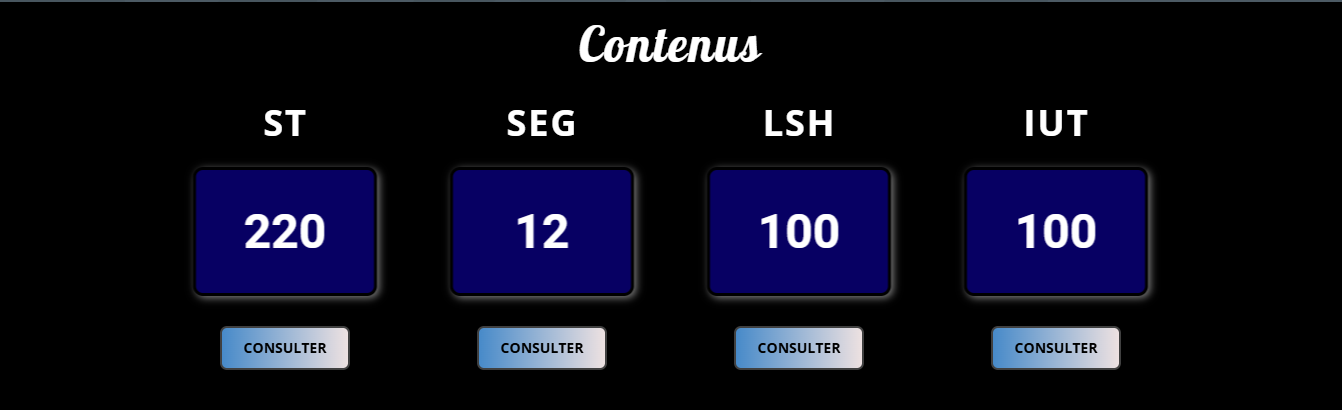
\includegraphics[width=16cm,height=9cm]{images/p1s2.PNG}%
    }
    \caption{Section pour le nombre de ressources disponible par UFR sur la plateforme }%
\end{figure}
\par

\textbf{Section 3 :}
A la troisième section nous avons les différents enseignants encadreur. Elle a pour but de permettre une meilleur indication concernant les noms des encadreurs figurant sur les travaux

\begin{figure}[H]%
    \center%
    \setlength{\fboxsep}{5pt}%
    \setlength{\fboxrule}{0.5pt}%
    \fbox{
    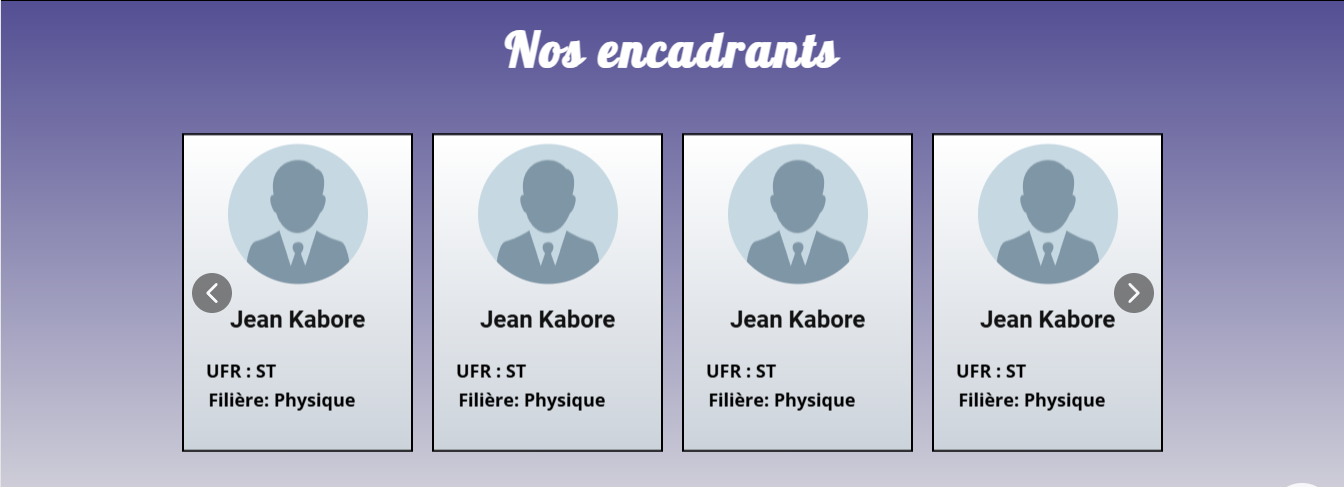
\includegraphics[width=16cm,height=9cm]{images/p1S3.PNG}%
    }
    \caption{Section pour les encadrants}%
\end{figure}
\par


\subsection{Liste des ressources}
Cette page présente la liste de ressources pour la catégorie sélectionné.

\begin{figure}[H]%
    \center%
    \setlength{\fboxsep}{5pt}%
    \setlength{\fboxrule}{0.5pt}%
    \fbox{
    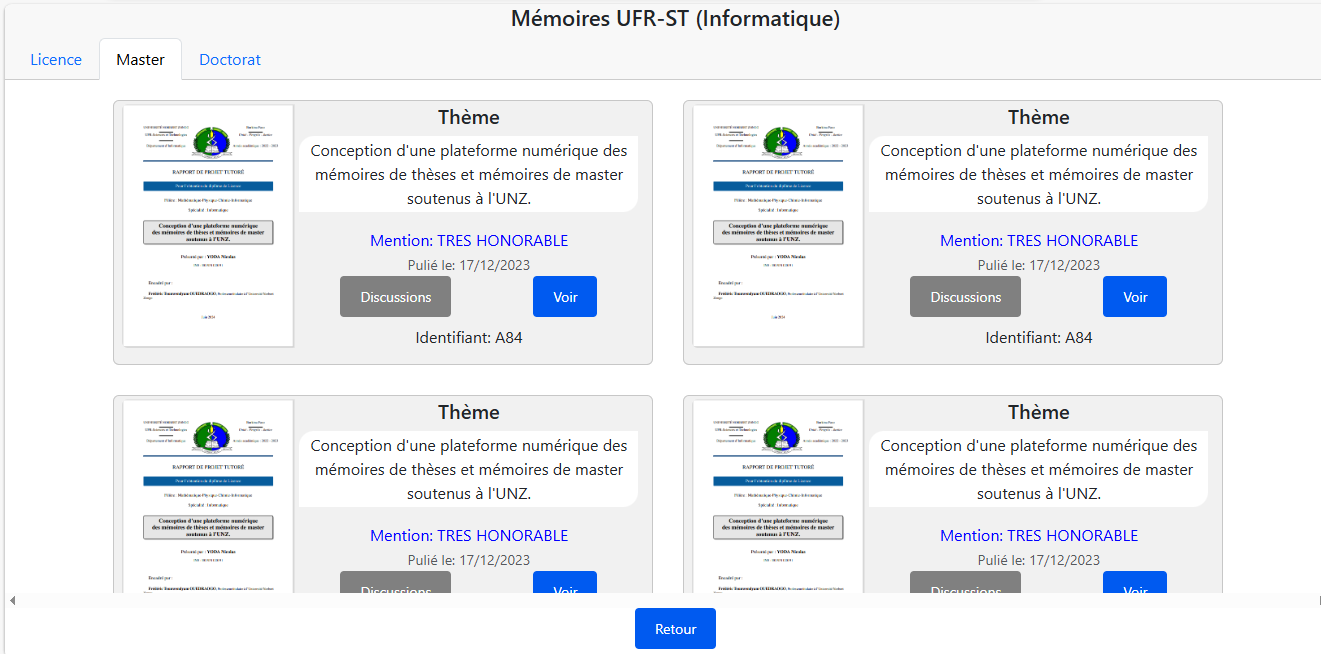
\includegraphics[width=16cm,height=9cm]{images/ressources.PNG}%
    }
    \caption{Liste des ressources}%
\end{figure}

\subsection{Formulaire de préoccupation}
Cette page présente le formulaire permettant aux utilisateurs de saisir leur préoccupation.

\begin{figure}[H]%
    \center%
    \setlength{\fboxsep}{5pt}%
    \setlength{\fboxrule}{0.5pt}%
    \fbox{
    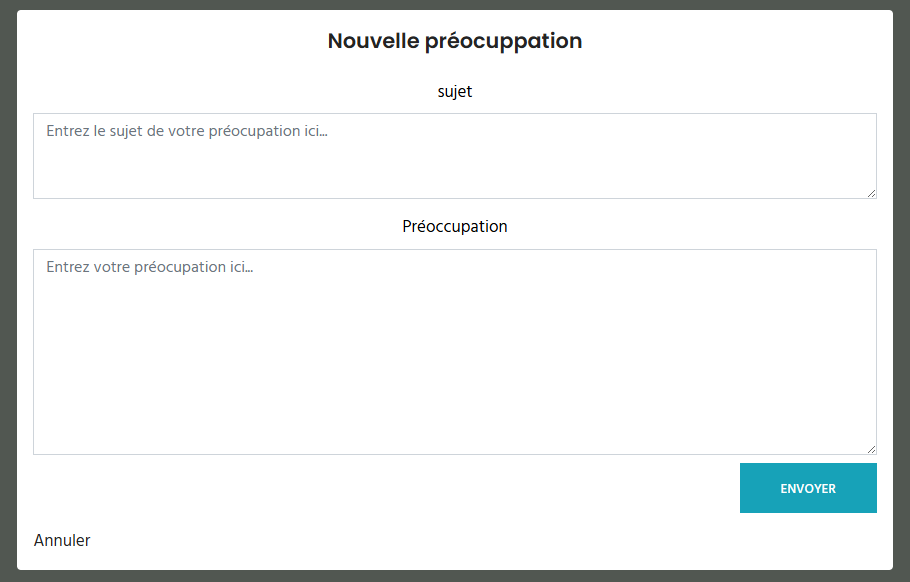
\includegraphics[width=16cm,height=9cm]{images/preocupation.PNG}%
    }
    \caption{Formulaire des préoccupations}%
\end{figure}

\subsection{Liste des préoccupations}
Ici nou avons la liste des différentes préoccupation qui ont été posé et un lien menant à la discussion concernant chaque préoccupation.

\begin{figure}[H]%
    \center%
    \setlength{\fboxsep}{5pt}%
    \setlength{\fboxrule}{0.5pt}%
    \fbox{
    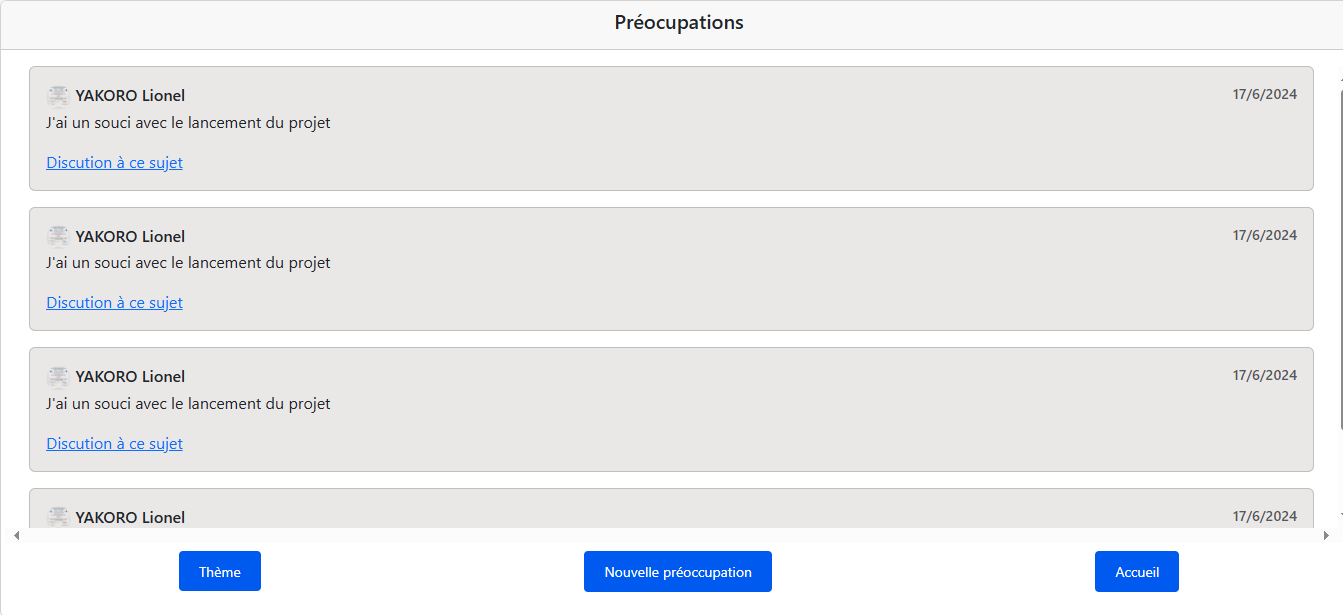
\includegraphics[width=16cm,height=9cm]{images/liste des preocupation.PNG}%
    }
    \caption{Liste des préoccupations}%
\end{figure}

\subsection*{Conclusion}
En conclusion nous pouvons affirmer que les différentes étapes de notre aventure nous ont permis de mettre en place une plateforme de 8 principales pages dénommée Bibliothèse.UNZ capable de stocker en ligne les mémoires de thèses et mémoires de master au format PDF et qui dispose de fonctionnalité de recherche ainsi qu'un cadre d'échange collaboratif entre les membres de la communauté universitaire.